\documentclass[11pt,american]{article}
\usepackage[T1]{fontenc}
\usepackage{babel}
\usepackage{csquotes}
\usepackage{amsmath}
\usepackage{graphicx}
\usepackage{amssymb}
\usepackage{tikz}
\usepackage{pgfplots}
 
\DeclareMathOperator{\const}{const}
\DeclareMathOperator{\sign}{sign}
\DeclareMathOperator{\atanh}{atanh}
\DeclareMathOperator{\R}{\mathbb{R}}
\DeclareMathOperator{\rank}{\operatorname{rank}}

\usepackage{color,ifpdf,graphicx}
\ifpdf %if using PDFTeX in PDF mode
  \DeclareGraphicsExtensions{.pdf,.png,.mps}
\else %if using TeX or PDFTeX in TeX mode
  \DeclareGraphicsExtensions{.eps,.bmp}
  \DeclareGraphicsRule{.emf}{bmp}{}{}% declare EMF filename extension
  \DeclareGraphicsRule{.png}{bmp}{}{}% declare PNG filename extension
  \usepackage{pstricks}%variant: \usepackage{pst-all}
\fi

\title{Trajectory tracking with singularities: homotopy continuation approach}
%\author{Alex Borisevich}

\begin{document}

\maketitle
This paper deals with a class of nonlinear MIMO system that is affine in input $u$

\begin{equation}
\dot x = f(x) + g(x) \cdot u, \; y = h(x)
\end{equation}

where $x \in \R^n$ and $u,y \in \R^m$.

TODO:

\section{Motivating example}

Let's consider very simple system that is just 

\begin{equation}\label{toy_example}
\dot x = u, \; y = h(x) = x \cdot (x^2 - 1)
\end{equation}

\begin{tikzpicture}
\begin{axis}[
    axis lines = center,
    xlabel = $x$,
    ylabel = {$h(x)$},
]
%Below the red parabola is defined
\addplot [
    domain=-1.5:1.5, 
    samples=100, 
    color=red,
]
{x*(x*x - 1)};
\addlegendentry{$x \cdot (x^2 - 1)$}
%Here the blue parabola is defined
%\addplot [
%    domain=-10:10, 
%    samples=100, 
%    color=blue,
%    ]
%    {x^2 + 2*x + 1};
%\addlegendentry{$x^2 + 2x + 1$}

\end{axis}
\end{tikzpicture}

The particular nonlinearity $h$ appears in some real word-applications like I-V curve of a tunnel diode.

From the control point of view, the system should be output controllable since any value of $y \in \R$ is reachable by substituting corresponding value of $x$.
However, from the linearization point of view, the $h$ has two singular points that prevent the system from linearization:

\begin{equation}
\frac{\partial h}{\partial x} = 3 x^2 - 1 = 0 
\end{equation}

And the slope of $h$ is negative between the singular points $x = \pm 1/\sqrt{3} \approx \pm 0.577$ while it is positive everywhere else.

\section{Well-behaving functions}

In this paragraph we recall trivial case when a function $f: \R^n \to \R^n$ under consideration is locally invertible in a domain of interest $x \in S$:

\begin{equation}
\rank D f(x) = n
\end{equation}

\subsection{Root-finding}

If the problem is to find a root of this function such that

\begin{equation}
f(x^*) = 0
\end{equation}

then a time derivative of $y = f(x)$ could be found:

\begin{equation}
\dot y = D f(x) \cdot \dot x
\end{equation}

and then the trajectory of $y$ could be designed such that $y(t) \to 0$ for example:

\begin{equation}
\dot y = -y
\end{equation}

or solving for $\dot x$:

\begin{equation}
\dot x = \Bigl[ D f(x) \Bigr]^{-1} \cdot \dot y = -\Bigl[ D f(x) \Bigr]^{-1} y
\end{equation}

The above is just well-known Newton's method written in continuous time.

\subsection{Trajectory tracking}

Generalizing the above approach, it is possible to follow an arbitrary smooth trajectory $y^*(t)$ by manipulating $\dot x$ through the invertible Jacobian matrix $D f(x)$ as 

\begin{equation}\label{newton_track}
\quad \dot x = \Bigl[ D f(x) \Bigr]^{-1} \cdot \dot y^*
\end{equation}

assuming $y(0) = y^*(0)$ without losing generality (the initial point $x_0$ for $f(x_0) = y^*(0)$ could be found by Newton's method described in previous section).


\section{Homotopy continuation}

Homotopy continuation (often called path following or continuation methods) is a family of numerical techniques primarily used to find solutions (roots) of systems of nonlinear equations. The central idea is to start with a system of equations whose solutions are known (or easy to obtain) and then continuously “morph” or deform that system into the one you’re interested in. By tracking how the solutions move under this continuous deformation (the “homotopy”), one can often locate the solutions of the target system.
Solutions can pass through singularities where standard methods as Newton's method breaks down unless carefully handled.

\subsection{Newton homotopy for root-finding}

Lets consider a nonlinear equation 

\begin{equation}
f(x) = y^*
\end{equation}

where $x^n \in R$ and $f: \R^n \to \R^n$.

A particular form of Newton homotopy for a problem $f(x) = y^*$ can be written as:

\begin{align}\label{hom_func}
H(x,\lambda) &= (1 - \lambda) \cdot \Bigl[ f(x) - f(x_0) \Bigr] + \lambda \cdot \Bigl[ f(x) - y^* \Bigr] \\
&= f(x) - f(x_0) + \lambda \cdot \Bigl[ f(x_0) - y^* \Bigr] 
\end{align}

where $x(0) = x_0$, and $\lambda \in \R$, $\lambda(0) = 0$, $\lambda \in [0,1]$.

The system $H = 0$ depends on a parameter $\lambda$ that evolves in time and the solution $x$ varies correspondingly to trace a curve $(x, \lambda)$ defined by $H(x, \lambda) = 0$.
For initial moment of time $t = 0$, $\lambda(0) = 0$ and $x(0) = x_0$ and $H(x_0,0) = 0$.

Typical assumption for the family of homotopy continuation methods is that the Jacobian of $H$ is a full rank matrix

\begin{equation}\label{full_rank_H}
\rank D H = n
\end{equation}

Worth noting that this requirement is more relaxed compared with just $\rank D f(x) = n$ as the $D H$ is $n\times(n+1)$ matrix and usually introducing additional degree of freedom $\lambda$ and column $n+1$ makes the $D H$ easier to invert in the augmented vector space $\R^{n+1}$.

One might try to step $\lambda$ from 0 to 1 directly, but that can fail if the solution curve folds in $\lambda$.  
Another approach is arc‐length (or pseudo‐arclength) continuation: it introduces a new parameter $s$ which is a curve arc-lendth and it could be considered as time $t$ if the curve is parameterized at unit speed. Also the method normalizes the tangent vector to the solution curve.

In arc‐length form, the solution curve

\begin{equation}
c(t) \;=\; (x(t),\,\lambda(t))
\end{equation}

lives in $\mathbb{R}^{n+1}$. The $c(t)$ is a solution of initial value problem defined by the following conditions (see Allgower \& Georg, Theorem/Lemma 2.1.6) :

1. $ \dot H\bigl(c(t)\bigr) \cdot \dot{c}(t) = 0$, (path following condition).

2. $\|\dot{c}(t)\| = 1$, (normalization condition).

3. $\det \begin{pmatrix} D H \\ \dot{c}^T \end{pmatrix} > 0$, (orientation condition).

It is easy to see that $H(x(0),\lambda(0))=H(x_0,0) = 0$ by defenition of the $H$. Thus imposing $\dot H = 0$ for the trajectory of $(x(t),\,\lambda(t))$ ensures that $H = \const = 0$.

Direct calculation of time derivative $\dot H$ of \eqref{hom_func} gives:

\begin{align}\label{diff_hom_func}
\dot H(x,\lambda) &= D f(x) \cdot \dot x + \bigl[ f(x_0) - y^* \bigr] \cdot \dot \lambda \\
&= \bigl[ D f(x) \; \big| \; f(x_0) - y^* \bigr] \cdot \begin{pmatrix} \dot x \\ \dot \lambda \end{pmatrix}
\end{align}

\subsection{Well-behaving function behaviour}

Consider a well-behaving function $f(x)$ in terms of $\rank D f(x) = n$ so that the $D f(x)$ is an invertible matrix. This consideration is important since by Sard's theorem that the set of critical values (that is, the image of the set of critical points where Jacobian is not full rank $\rank D f(x) < n$) of a smooth function $f$ from one Euclidean space or manifold to another is a null set. Thus a function $f$ is almost everywhere in its domain is a well-behaving function.

If $\rank D f(x) = n$ then it is possible to can mulitply the \eqref{diff_hom_func} by $\Bigl[ D f(x) \Bigr]^{-1}$ and obtain $\dot x$ as a function of $\dot \lambda$:

\begin{gather}
\dot H(x,\lambda) = \dot x + \Bigl[ D f(x) \Bigr]^{-1} \bigl[ f(x_0) - y^* \bigr] \cdot \dot \lambda = 0\\
\dot x = \Bigl[ D f(x) \Bigr]^{-1} \bigl[ y^* - f(x_0) \bigr] \cdot \dot \lambda = A^{-1} u \cdot \dot \lambda
\end{gather}

where $A = D f(x)$, $u = f(x_0) - y^*$.

Then it is possible to employ normalization condition 2 for the arc-lendth continuation initial value problem: 

\begin{gather}
\|(\dot x,\dot \lambda)\| = 1 \\
\|(\dot x,\dot \lambda)\|^2 = 1 \\
\| ( A^{-1} u \cdot \dot \lambda , \dot \lambda ) \|^2 = 1 \\
(\dot \lambda)^2 \cdot \| (A^{-1} u , 1) \|^2 = 1 \\
(\dot \lambda)^2 \cdot \Bigl( \| A^{-1} u \|^2 + 1 \Bigr ) = 1
\end{gather}

So

\begin{equation}
\dot \lambda = \pm \frac{1}{\sqrt{\|A^{-1}u\|^2 + 1}}.
\end{equation}

Due to orientation condition 3 of the arc-lendth continuation method we need to pick $+$ sign for the $\dot \lambda$:

\begin{gather}
\dot \lambda = \frac{1}{\sqrt{\|A^{-1}u\|^2 + 1}}.
\end{gather}

The dynamics of $\dot x$ and $\dot \lambda$ in the original notation:

\begin{gather}
\dot x = \alpha \cdot \Bigl[ D f(x) \Bigr]^{-1} \bigl[ y^* - f(x_0) \bigr] \\
\dot \lambda = \alpha
\end{gather}

where normalization factor $\alpha$ is

\begin{equation}
\alpha(x) = \frac{1}{\sqrt{\left\| \Bigl[ D f(x) \Bigr]^{-1} \bigl[ y^* - f(x_0) \bigr] \right\|^2 + 1}}
\end{equation}

The resulting dynamics of $y$ could be found by computing time derivative of $y = f(x)$:

\begin{equation}
\dot y = D f(x) \cdot \dot x = \alpha \cdot \bigl[ y^* - f(x_0) \bigr]
\end{equation}

So $y$ is linearly moving from $f(x_0)$ to $y^*$ along the vector $y^* - f(x_0)$ with the rate of $\alpha(x) > 0$.

\subsection{Bifurcation points}

It is known that if $\rank D f(x) = n - 1$ then the curve $H(x,\lambda) = 0$ exhibits either inflection point or turning point.
If $H(x,\lambda)$ 

TODO:

\section{Nonlinear trajectory tracking}

Let's consider a problem of following a trajectory $y(t) = y^*(t)$. 

\subsection{Descrete and continous time problem formulations}

A practical approach to this problem would be approximating the $y^*(t)$ with a series of subproblems involving discrete points $y^*_k$ sampled along the trajectory $ y^*_k = y^*(k \Delta T) $ at intervals $ \Delta T $. The continuous trajectory-following problem is then decomposed into a series of subproblems, each involving reaching to the discrete point $y(k \Delta T) = y^*_k$ at time $ t_k = k \Delta T $, $k \ge 1$.

The process starts at $x_0$ and $y_1$ should be attended which was sampled at moment $t_1$, and then it start again at $x_1$ for which $f(x_1)=y_1$ to attend $y_2$ sampled at the moment of $t_2$ etc.
 
The homotopy function \eqref{hom_func} to attend $y_{k+1}$ can be written as

\begin{equation}
H_k(x,\lambda) = f(x) - f(x_k) + \lambda \cdot \Bigl[ f(x_k) - y^*_{k+1} \Bigr] 
\end{equation}

where parameter $\lambda$ starts with 0 and ends with 1 every iteration $k$.

It is more convenient to consider a continously increasing parameter $\mu$ that is related to $\lambda$ as:

\begin{equation}
\lambda = \mu - t_{k+1} + 1
\end{equation}

and the range of $\mu$ in every iteration $k$ is $[t_{k+1} - 1, t_{k+1}]$ so the $\lambda$ is still between $[0,1]$.

The homotopy function then can be reformlated as:

\begin{equation}
H_k(x,\mu) = f(x) - f(x_k) + (\mu - t_{k+1} + 1) \cdot \Bigl[ f(x_k) - y^*_{k+1} \Bigr] 
\end{equation}

The newly introduced parameter $\mu$ starts every iteration from $\mu(t_k) = t_{k+1} - 1$ and finishes at $\mu(t_{k+1}) = t_{k+1}$ so the

\begin{gather}
H_k(x,\mu(t_k)) = f(x) - f(x_k) \\
H_k(x,\mu(t_{k+1})) = f(x) - y^*_{k+1}
\end{gather}

The following of the curve $H_k(x,\mu) = 0$ should bring the $f(x)$ from point $y^*_k = f(x_k)$ to $y^*_{k+1} = f(x_{k+1})$.

It is obvious to see that for every moment of time $t_k$ when a reference point $f(x_k) = y^*_k$ is attended the value $\mu$ is syncronized with time $\mu(t_k) = t_k$.

In a situation when the trajectory $y^*(t)$ is followed closely one would expect that the $y^*(t)$ is sampled with a very small time stamp $\Delta T \to 0$ and there is infinitesimal difference between adjacent time stamps $t_k$ and $t_{k+1}$. In this case it is possible to formulate a continous time trajectory tracking problem with the following homotopy function:

\begin{equation}\label{hom_tracking}
H(x,\mu, t) = f(x) - f(x_0) + (\mu - t + 1) \cdot \Bigl[ f(x_0) - y^*(t) \Bigr] 
\end{equation}

where $x_0$ is a starting point of the trajectory $x(t)$: $x_0=x(t)$.

If $f(x_0) \ne y^*(0)$ then $\mu(0) = -1$, otherwise if the $f(x_0)$ is already on the reference trajectory the initial transient can be ommited having $\mu(0)=0$.

The time derivative of $H$ is

\begin{equation}\label{diff_hom_tracking}
\dot H = D f(x) \cdot \dot x + (\dot {\mu} - 1)\Bigl[ f(x_0) - y^*(t) \Bigr] - (\mu - t + 1) \cdot \dot y^*(t)
\end{equation}

It is easy to see that in order to track the $y^*(t)$ exactly the following has to be true 

\begin{gather}
f(x) - y^*(t) = 0 \\
D f(x) \cdot \dot x - \dot y^*(t) = 0
\end{gather}

which is only possible with

\begin{equation}\label{tracking_conditions}
\mu = t, \quad \dot {\mu} = 1
\end{equation}

Thus in an ideal situation of tracking a well-behaving function that has invertible $D f(x)$, the parameter $\mu$ is simply time $t$.
But generally $\mu$ is allowed to deviate from time $t$ to ovecome singularities of $f(x)$.

\subsection{Problem solution}

In this section we are going to follow the approach developed in [].

Below is a block-structure viewpoint of the Jacobian $D H(x,\mu,t)$ for the particular homotopy function \eqref{hom_tracking}.

We'll split the Jacobian into two main blocks:  

- A: the block corresponding to partial derivatives w.r.t. $(x,\mu)$, which is $n \times (n+1)$ matrix.  

- B: the block (column) corresponding to partial derivatives w.r.t. $t$, which is $n \times 1$ column-vector.

In symbols:

\[
\underbrace{A}_{n\times(n+1)}
\;=\;
\begin{pmatrix}
\dfrac{\partial H}{\partial x} & \dfrac{\partial H}{\partial \mu}
\end{pmatrix} = D_{x,\mu} H,
\quad
\underbrace{B}_{n\times1}
\;=\;
\dfrac{\partial H}{\partial t}.
\]

Hence,
\[
DH(x,\mu,t) 
\;=\;
\bigl[A \;\big|\; B\bigr]
\;\in\;\mathbb{R}^{n\times(n+2)}.
\]

We are going to impose a condition similar to the \eqref{full_rank_H} for invertibility of the block $A$ of the Jacobian

\begin{equation}\label{full_rank_A}
\rank A = \rank D_{x,\mu} H = n
\end{equation}

As for the \eqref{full_rank_H} this is indeed a weaker condition compared with $\rank D f = n$ as it could be that the $\rank D_{x,\mu} H = n$ even if the $\rank D f = n - 1$.

Geometrically or numerically \eqref{full_rank_A} implies that, at the point in question, one can (locally) solve

\[
H(x,\mu,t)\;=\;0
\quad\text{for $\,(x,\mu)$\, given a small change in $t$.}
\]

Because if $A$ has rank $n$, it is possible to invert the linear map from $(\delta x,\,\delta\mu)\mapsto A\,(\delta x,\,\delta\mu)$ at least in a one-dimensional sense (there is exactly one missing dimension corresponding to the fact that $A$ is $n\times(n+1)$). 

Concretely:

1. Dimensionality: we have $n$ equations in $\{H=0\}$ but $n+2$ unknowns $(x,\mu,t)$.
  
2. Rank Condition: if $\mathrm{rank}(A)=n$, we can (locally) treat $(x,\mu)$ as implicit functions of $t$.  

If that rank condition fails, we are at singular or critical point with respect to $(x,\mu)$, and special handling may be required to continue solutions in $(x,\mu,t)$-space.

The $B = \partial H/\partial t$ is the $n\times1$ partial derivative of the homotopy with respect to the time $t$.

In a continuation viewpoint, if one wants to track $\bigl(x(t),\,\mu(t)\bigr)$ as $t$ changes, the condition

\[
H\bigl(x(t),\mu(t),t\bigr)\;=\;0
\]

plus the chain rule leads to

\[
\dot H = A \cdot \dot c + B = 0.
\]

where

\[
\dot c(t) = \begin{pmatrix} \dot{x}(t) \\ \dot{\mu}(t) \end{pmatrix}
\]
  
If $\mathrm{rank}(A)=n$, one can solve for $(\dot{x}(t),\,\dot{\mu}(t))$ substituting $\dot{t} = 1$.  

Hence, in differential-algebraic terms

\[
\underbrace{\begin{pmatrix}
\frac{\partial H}{\partial x} & \frac{\partial H}{\partial \mu}
\end{pmatrix}}_{=A}
\begin{pmatrix}
\dot{x}(t)\\[4pt]
\dot{\mu}(t)
\end{pmatrix}
\;+\;
\underbrace{\frac{\partial H}{\partial t}}_{=B}\
\;=\;
0
\]

that gives a solution

\begin{equation}\label{solution_drift}
\dot c_p = -A^\dagger\,B\,
\end{equation}

where $A^\dagger$ is a right-inverse of $A$ (possible because $\rank A=n$).

The geometric interpretation of the result above is:

1. Constraint $H(x,\lambda,t)=0$ defines an $(n+1)$-dimensional manifold in $\mathbb{R}^{n+2}$ (assuming it’s regular). 
 
2. By setting $\dot{t}=1$ a particular slice in the parameter $(x,\lambda)$-space for each increment of $t$ is chosen.  

3. The drift term $\partial H/\partial t$ represents how $H$ changes with time $t$ alone. In order to remain on $H=0$, the $(x,\lambda)$ must counteract that drift. That’s precisely what solving $A \cdot \dot c = -B$ does. Hence, once $A$ has a left inverse, we can cancel out or neutralize the effect of $B$.

It is important to understand that the solution $\dot c_p$ per \eqref{solution_drift} is not unique as the $A$ is a non-square $ n \times (n+1) $ matrix.
Since $ A $ has full row rank by the assumption \eqref{full_rank_A} then the null space of $ A $ has dimension $ (n+1) - n = 1 $, meaning there is a single linearly independent vector in the null space. 

In this case, the general solution can be written as 

\begin{equation}\label{solution}
\dot c = -A^\dagger\,B + \gamma \cdot \ker(A) = \dot c_p + \gamma \cdot \dot c_h
\end{equation}

where:

- $\dot c_p$ is a particular solution of the $A \cdot \dot c = -B$ per \eqref{solution_drift}.

- $\dot c_h$ is a basis vector for the null space (kernel) of $A$ which can be obtained as the last column of the orthogonal matrix $Q$ from the QR decomposition of $A^T$.

- $\gamma$ is a free scalar parameter.

In order to select a unique solution for $\dot c$ we have to impose an additional constraint. Following the arc‐length continuation methods, the additional conditions to uniquely determine the curve $x(t),\,\mu(t))$ are normalization and orientation conditions:

\begin{equation}\label{conditions}
\begin{gathered}
\| \dot{c_h} \| = 1, \\
\det \begin{pmatrix} A \\ \dot{c_h}^T \end{pmatrix} > 0
\end{gathered}
\end{equation}

The solution \eqref{solution} together with conditions \eqref{conditions} determine unique solution trajectory of the homotopy equation $H(x(t),\mu(t),t)=0$ assuming $H(x(0),\mu(0),0)=0$. This result however doesn't guarantee tracking of a trajectory $y^*(t)$ for a particular homotopy function \eqref{hom_tracking}. The next section solves this.

\subsection{Accuracy of tracking}
 
Generally, the conditinos \eqref{tracking_conditions} may not be satisfied everywhere since the reference trajectory $y^*(t)$ is not exactly tracked. Particularly in two cases: if the $x_0$ doesn't lie on the $y^*(t)$ such there is an initial transient to reach the $y^*(t)$, or if the trajectory tracking requires overcoming singular points of $f(x)$.

It is expected to minimize a following type of criteria to ensure accuracy of the trajectory tracking
  
\begin{equation}\label{objective}
\int_0^T \| f(x(t)) - y^*(t) \|^2 dt \to \min
\end{equation}

where $\| v \|^2 = v^T v$.

It is easy to see that minimizing the error $e = t - \mu$ implies minimizing the \eqref{objective}. 

\begin{equation}
\int_0^T \bigl[ t - \mu(t) \bigr]^2 dt \to \min  \implies  \int_0^T \| f(x(t)) - y^*(t) \|^2 dt \to \min
\end{equation}

The \eqref{hom_tracking} can be rearranged as

\begin{equation}
H(x,\mu, t) = f(x) - y^*(t) + (\mu - t) \cdot \Bigl[ f(x_0) - y^*(t) \Bigr] 
\end{equation}

So satisfying $H = 0$ means

\begin{equation}
f(x) - y^*(t) = (t - \mu) \cdot \Bigl[ f(x_0) - y^*(t) \Bigr] 
\end{equation}

thus

\begin{equation}
\int_0^T \| f(x) - y^*(t) \|^2 dt = \int_0^T \bigl[ t - \mu(t) \bigr]^2 \cdot \| f(x_0) - y^*(t) \|^2 dt
\end{equation}

If $y^*(t)$ is bounded around $f(x_0)$ as it lies inside of a ball of radius $M$ centered at $f(x_0)$, i.e. $\|f(x_0) - y^*(t)\| < M$ then

\begin{gather}
\int_0^T \| f(x) - y^*(t) \|^2 dt = \int_0^T \bigl[ t - \mu(t) \bigr]^2 \cdot \| f(x_0) - y^*(t) \|^2 dt \\
< M^2 \int_0^T \bigl[ t - \mu(t) \bigr]^2 dt
\end{gather}

The solution \eqref{solution} has an additional degree of freedom $\gamma$ that can be used to force the trajectory $\mu(t)$ converge to $t$. 

If 

\begin{equation}
e(t) = t - \mu(t)
\end{equation}

and

\begin{equation}
\gamma = k \cdot e(t)
\end{equation}

then for a sufficiently large scalar constant $k > 0 > m$ the error $e(t)$ is bounded $|e(t)| < \epsilon$.

Let's define block matrices $A$ and $B$ for the particuar homotopy function under consideration \eqref{diff_hom_tracking} as

\begin{equation}\label{conditions}
\begin{gathered}
A = \begin{pmatrix}
D f(x) & f(x_0) - y^*(t)
\end{pmatrix} \\
B = y^*(t) - f(x_0) - (\mu - t + 1) \cdot \dot y^*(t)
\end{gathered}
\end{equation}

Let's consider behaviour away from singularities where function $f(x)$ is well-behaving in terms of $\rank D f(x)=n$ and where the $y^*(t)$ can be exactly tracked.
In this case a particular form of the right inverse $A^\dagger$ of the matrix $A$ is simply:

\begin{equation}
A^\dagger = \begin{pmatrix}
\Bigl[ D f(x) \Bigr]^{-1} \\ 0
\end{pmatrix}
\end{equation}

Thus the dynamics of $\mu(t)$ is fully driven by the homogeneous part solution:

\begin{equation}
\begin{pmatrix} \dot{x}(t) \\ \dot{\mu}(t) \end{pmatrix} = \gamma \cdot \ker(A)
\end{equation}

also subject to additional constraints \eqref{conditions}.

The kernel of the matrix $A$ has the following closed form as the $D f(x)$ is invertible:

\begin{equation}
\ker(A) = \begin{pmatrix}
\Bigl[ - D f(x) \Bigr]^{-1} \cdot (f(x_0) - y^*(t)) \\ 1
\end{pmatrix}
\end{equation}

So as expected, the solution trajectory by the \eqref{solution} for \eqref{diff_hom_tracking} with unity scaling $\gamma = 1$ produced $\dot \mu = 1$.
Now if $\gamma = k \cdot [t - \mu(t)]$ the final dynamic is

\begin{equation}
\dot \mu = k \cdot [t - \mu(t)]
\end{equation}

the solution with the initial condition is

\begin{equation}
\mu(t) = t - \frac{1}{k} + \Bigl(\mu(0)+\frac{1}{k}\Bigr) \cdot e^{-kt} \to t - \frac{1}{k}
\end{equation}

Thus for $t \to \infty$ the $\mu(t)$ follows $t$ up to to $-1/k$, so for $k$ the asymptotic tracking error is

\begin{equation}
|e(t)| = |t - \mu(t)| \le 1/k
\end{equation}


\section{Numerical simulations}

Let's consider a problem of tracking the reference $y^*(t) = -6 \cos(t)$ by a toy example \eqref{toy_example} given as a function $h(x) = x (x^2 - 1)$.
The simulations obtained with $k = 100$.

\begin{center}
\ifpdf %if using PDFTeX in PDF mode
  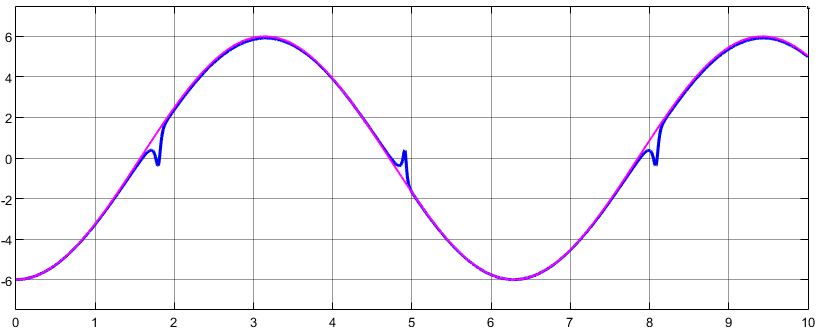
\includegraphics[width=1\textwidth]{toy_y.png}
\fi

Figure 1. Dynamics of the function $f(x(t))$ (blue) tracking the reference $y^*(t)$ (red).
\end{center}

\begin{center}
\ifpdf %if using PDFTeX in PDF mode
  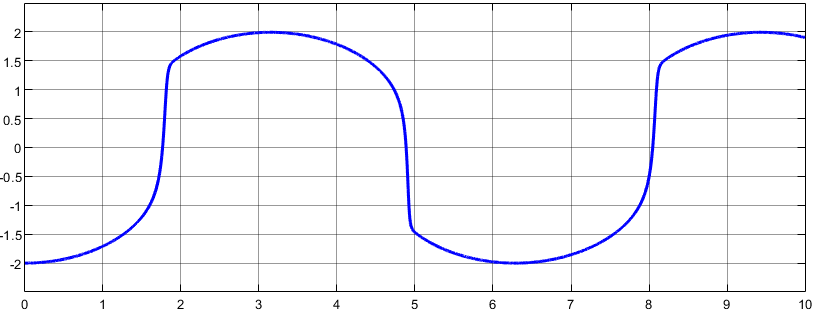
\includegraphics[width=1\textwidth]{toy_x.png}
\fi

Figure 2. Dynamics of the function argument $x(t)$.
\end{center}

\begin{center}
\ifpdf %if using PDFTeX in PDF mode
  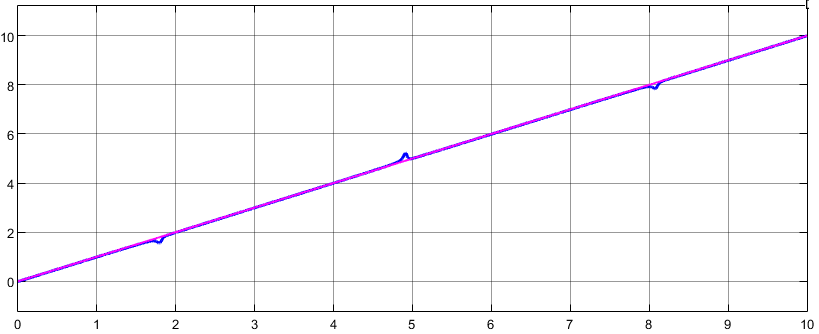
\includegraphics[width=1\textwidth]{toy_mu.png}
\fi

Figure 3. Dynamics of the parameter $\mu$ (blue) compared with time $t$ (red).
\end{center}

\end{document}




